\documentclass[a4paper,12pt]{article}

\usepackage[utf8]{inputenc}
\usepackage[T1]{fontenc}
\usepackage{amsmath}
\usepackage{amssymb}
\usepackage{graphicx}
\usepackage{hyperref}
\usepackage{geometry}
\usepackage[italian]{babel}
\usepackage{svg}
\usepackage{float}
\usepackage{enumitem}

\geometry{a4paper, margin=1in}



\title{Progetto di Algoritmi e Protocolli per la Sicurezza}
\author{Davide D'Acunto\quad Noemi Biancamano}
\date{Gruppo 9}
\begin{document}

\maketitle

\tableofcontents
\newpage
\section{WP 1: Modello}
La seguente sezione si occupa di descrivere gli attori onesti presenti nel sistema, evidenziando le attività che sono interessati a svolgere.
\newline Successivamente, si procede alla discussione degli avversari e del threat model considerato, andando a specificare le capacità e le risorse da essi possedute. Infine, si presentano le proprietà che devono essere preservate dal sistema al fine di essere resiliente agli attacchi considerati.
\subsection{Attori \& Obiettivi}
\begin{figure}[H]
    \centering
    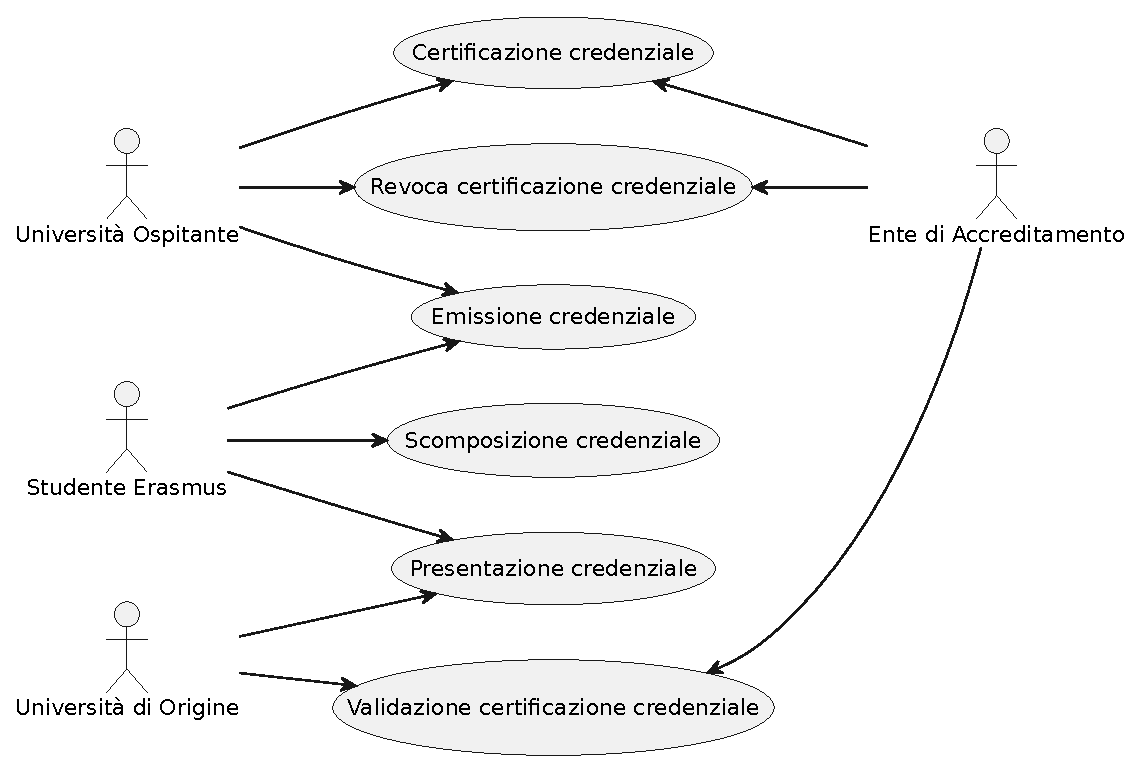
\includegraphics[width=0.95\textwidth]{usecase_1.eps}
    \caption{Use Case degli attori onesti}
    \label{fig:usecase1}
    
\end{figure}
\subsubsection{Studente Erasmus}
Lo studente Erasmus è interessato a sostenere attività accademiche all'interno della sede ospitante, le quali devono essere poi certificate e dimostrate all'università di origine.
\paragraph{Richiesta credenziale} Lo studente deve ricevere dall'università ospitante una credenziale accademica, che attesti le attività da egli effettuate durante il periodo di mobilità.
\paragraph{Trasmissione credenziale} Tale credenziale dev'essere successivamente fornita all'università di origine per certificare le attività svolte dallo studente nella sede ospitante. 
\paragraph{Condivisione selettiva} Lo studente potrebbe desiderare di comunicare solamente un sottoinsieme strettamente necessario delle informazioni contenute all'interno della credenziale, in maniera tale da dimostrare il rispetto dei criteri dell'accordo di mobilità e non rivelare informazioni personali superflue.
\\[0.5em] Si suppone che le risorse computazionali dello studente siano limitate. 

\subsubsection{Università Ospitante}
L'università ospitante, accordatasi con l'università di origine, permette a vari studenti Erasmus di poter usufruire di un periodo di mobilità all'interno della sua sede, nel quale gli studenti hanno la possibilità di effettuare varie atttività accademiche.
\paragraph{Emissione credenziale} La sede è interessata a certificare, per ogni studente in mobilità da essa, le attività svolte da questo attraverso una credenziale, cosicché egli sia in grado di comunicarle successivamente alla sua sede d'origine.
\paragraph{Interoperabilità credenziale} Siccome l'università ospitante non conosce i criteri definiti dall'accordo di mobilità per ciascuno degli studenti, inserisce nelle credenziali tutte le informazioni relative alle attività accademiche dello studente, sicché sia poi in grado di poterle comunicare all'università di origine. Tutte le informazioni devono essere rappresentate in un formato standard, definito congiuntamente con l'università di origine, per garantire l'interoperabilità delle credenziali.
\paragraph{Certificazione credenziale} L'ateneo desidera dimostrare che la credenziale è stata effettivamente emessa da sé, per cui rilascia un certificato dell'avvenuta emissione.
\paragraph{Revoca certificazione} In particolari casi laddove si verifichino: errori amministrativi, lo studente fornisce dati fraudolenti, comette plagio, oppure frode, e altre situazioni simili, l'università ospitante deve essere in grado di invalidare la credenziale revocandone il certificato.
\paragraph{Certificato pubblico} L'università ospitante deve contattare un ente di accreditamento per richiedere un certificato, il quale attesti l'autenticità delle sue comunicazioni, e le permetta di rilasciare certificazioni valide.
% \\[0.5em]Si suppone che le università ospitanti possiedano medie o elevate risorse computazionali.

\subsubsection{Università di Origine}
L'università di origine è accordata con l'università ospitante, mentre con lo studente attraverso un accordo di mobilità. All'interno di questo vengono definite tutte le attività accademiche che allo studente è richiesto soddisfare per validare il suo periodo di mobilità.
\paragraph{Presentazione credenziale} L'ateneo si aspetta di ricevere, da ciascuno studente che ha terminato il proprio periodo di mobilità, una credenziale nella quale sono presenti almeno le attività definite dall'accordo di mobilità.
\paragraph{Validazione credenziale} La credenziale deve essere certificata dall'università ospitante, cosicché si abbia la certezza della validità di questa. Qualora la credenziale non fosse certificata, invalida oppure revocata, l'ateneo è in grado di rifiutare la credenziale.
\paragraph{Verifica certificato} L'università di origine deve poter verificare l'autenticità della credenziale, attraverso la verifica del certificato associato ad essa.

\subsubsection{Ente di accreditamento}
L'ente di accreditamento è un'autorità esterna, che si occupa di certificare le università, in modo tale da garantire l'autenticità delle comunicazioni. 
\paragraph{Emissione certificato} L'ente di accreditamento emette certificati per le università che lo richiedono, i quali vengono utilizzati da queste per certificare o validare credenziali.
\paragraph{Archiviazione certificati} Non solo, si occupa anche dell'archiviazione delle certificazioni associate alle università, conservandole sino ad una determinata data, e rendendoli disponibili per la validazione.
\paragraph{Revoca certificato} L'ente di accreditamento deve essere in grado di revocare i certificati emessi, qualora vi siano errori o violazioni.

\subsection{Credenziale}
La credenziale è un documento contenente le informazioni relative alle attività accademiche che lo studente in mobilità ha svolto nella sede ospitante. 
\newline Le informazioni contenute all'interno della credenziale sono le seguenti:
\begin{itemize}
    \item Matricola interna dello studente
    \item Nome e cognome dello studente
    \item Matricola esterna dello studente
    \item Codice e nome dell'università ospitante
    \item Nome e cognome del referente dell'università di origine
    \item Nome e cognome del referente dell'università ospitante
    \item Data di emissione  
    \item Data di fine validità
    \item Periodo di mobilità
    \item Per ciascun esame sostenuto:
    \begin{itemize}[label=$\circ$]
        \item Nome e codice dell'esame
        \item Eventuale voto espresso in trentesimi, oppure esito
        \item Eventuale lode
        \item CFU conseguiti
        \item Data di superamento dell'esame
        \item Nome e cognome del docente
        \item Nome e codice del corso di laurea
    \end{itemize}
    \item Per ciascuna attività svolta:
    \begin{itemize}[label=$\circ$]
        \item Nome e codice dell'attività
        \item Periodo di inizio e fine dell'attività
        \item Eventuali CFU dell'attività
        \item Nome e cognome del docente o del referente
    \end{itemize}
\end{itemize}
Le università devono attenersi a questo formato per assicurare l'interoperabilità delle credenziali emesse.
\subsection{Threat Model}
Come threat model si considerano avversari che potrebbero compromettere il sistema con una determinata sequenza di azioni, le quali dipendono dalle risorse e capacità da essi possedute, definendo poi quale sia la proprietà che potrebbe venire meno laddove il sistema non sia resiliente a tale attacco.
\newline Ciascun attaccante viene considerato efficiente e probabilistico, ovvero con una determinata probabilità di avere successo nell'intento in tempo polinomiale.
\subsubsection{Violazione dell'ente di accreditamento}
Si prende in esame il caso in cui l'ente di accrediamento venga compromesso da un attaccante, il quale riesce ad ottenere accesso ai meccanismi di emissione e revoca dei certificati. In questo caso, l'attaccante potrebbe emettere certificati falsi, oppure revocare certificati validi.
\newline In questo caso si perde la proprietà di autenticità, in quanto non si ha la certezza che il certificato sia stato emesso da un'autorità competente, problema che si ripercuote sulle comunicazioni tra gli altri attori, siccome la loro fiducia nella sicurezza si basa sui certificati emessi.
\subsubsection{Violazione dell'università ospitante}
Si considera lo scenario dove l'università ospitante viene compromessa da un attaccante, il quale riesce ad ottenere accesso ai meccanismi di emissione, certificazione e revoca delle credenziali. In questo caso, l'attaccante diverrebbe in grado di:
\begin{itemize}
    \item Emettere credenziali false
    \item Certificare credenziali false
    \item Revocare certificazioni
\end{itemize}
In questo caso si perde la proprietà di autenticità, siccome non si ha la certezza che la certificazione sia stata emessa dall'università.
\subsubsection{Violazione dell'università di origine}
Si analizza il caso in cui l'università di origine venga compromessa da un attaccante, il quale riesce ad ottenere accesso ai meccanismi di validazione delle credenziali. In questo scenario, l'attaccante potrebbe accettare credenziali false, oppure respingere credenziali valide.
\newline Così si perde la proprietà di confidenzialità, poiché l'attaccante sarebbe in grado di accedere a informazioni riservate riguardanti studenti, attraverso le credenziali che inviano all'ateneo, ignari che sia stato violato.
\subsubsection{Studente malevolo}
Si studia il caso laddove lo studente sia malevolo, e tenti di far passare come valida una credenziale insufficiente, oppure alterata. In questo caso, lo studente 
\subsubsection{Intercettatore di comunicazioni dell'università ospitante}
Si prende in esame la presenza di un attaccante che intercetti tutte le comunicazioni da e verso l'università ospitante. Questo attaccante ha accesso a uno storico di messaggi cifrati e relative decifrature attraverso mezzi alternativi. 
\newline In questo caso, l'attaccante potrebbe essere in grado di inferire informazioni sui successivi messaggi cifrati, violando la proprietà di confidenzialità. Non solo, l'attaccante potrebbe alterare le comunicazioni in uscita, violando quindi le proprietà di sicurezza del sistema.
\subsubsection{Ascoltatore di comunicazioni dello studente}
Si prende in esame la circostanza di un attaccante che ascolti le comunicazioni tra studente ed altri attori, presente sul canale di comunicazione prima che questa avvenga. In questo caso, l'attaccante potrebbe carpire informazioni riservate, come la credenziale dello studente, violando la proprietà di integrità.
\subsubsection{Attacco con credenziale nota}
Si tiene in considerazione il caso di un attaccante che riesca ad ascoltare la conversazione tra l'università di origine e uno studente di cui conosce la credenzale attraverso altri mezzi.
\newline In questo caso, l'attaccante potrebbe inferire informazioni riguardati il meccanismo di comunicazione sicura, e violare le proprietà di sicurezza del sistema. 

\subsection{Proprietà}
In questa sezione si discuteranno con maggior riguardo le proprietà che il sistema deve possedere per soddisfare i requisiti di sicurezza richiesti.
\subsubsection{Confidenzialità}
Con confidenziale si intende l'accesso alle informazioni solamente a coloro che sono autorizzati. Nessun individuo non autorizzato deve accedere, neanche in parte, ad alcuna informazione che non è loro permesso di vedere.
\subsubsection{Integrità}
Con proprietà di integrità ci si riferisce alla garanzia che non vi siano alterazioni di messaggi durante la trasmissione. 
\subsubsection{Autenticità}
L'autenticità è la proprietà che assicura l'originalità del messaggio, ovvero che sia stato effettivamente inviato dal mittente, e che non ci sia stata alcuna impersonificazione.
\subsubsection{Revocabilità}
La revocabilità è l'abilità da parte di un ente certificatore di revocare una sua certificazione precedentemente emessa. Ciò richiede che l'ente informi tutti gli attori interessati di ciascuna revoca.
\subsubsection{Non ripudio}
La proprietà di non ripudio è la garanzia con la quale un attore non è in grado di negare di aver effettuato una certa azione. In questo caso, l'attore non è in grado di negare di aver emesso una credenziale.
\subsubsection{Interoperabilità}
L'interoperabilità è la proprietà che assicura che le credenziali emesse da un'università siano riconoscibili dalle altre università, a patto che rispettino un formato definito.
\subsubsection{Disponibilità}
La disponibilità è la proprietà che assicura continua operatività del sistema, ovvero che gli attori siano in grado di accedere e utilizzare il sistema in qualsiasi momento.
\subsubsection{Trasparenza}
La trasparenza è la proprietà attraverso la quale ciascun attore è sempre in grado di risalire all'autore di una data azione, possa essa essere l'emissione di un certificato, oppure la sua revoca.
\subsubsection{Scalabilità}
La proprietà di scalabilità garantisce che non vi sia riduzione delle prestazioni del sistema, all'aumentare dei nodi.
\subsubsection{Divulgazione selettiva}
Ciascuno studente deve poter essere in grado di divulgare soltanto un sottoinsieme strettamente necessario delle sue informazioni. Tale proprietà è denominata divulgazione selettiva.



\newpage
\section{WP 2}
\subsection{Introduzione alla soluzione}
In questa sezione si presenta la soluzione proposta per il modello descritto precedentemente.
\newline Nella prima sezione si descrive il sistema di certificazione delle università, il quale permetterà il rispetto della proprietà di autenticità, fondamentale per la parte successiva. In questa parte vengono trattate le interazioni tra le università e l'ente di accreditamento.  
\newline Segue l'esposizione del sistema di gestione dei certificati delle credenziali degli studenti, il quale si basa sull'utilizzo dei certificati per l'autenticazione delle università nel sistema. Le interazioni rappresentate sono quelle tra le università. 
\newline Infine, si spiega come lo studente possa utilizzare il sistema per validare le attività svolte durante il periodo di mobilità. Qui ricadono le interazioni tra lo studente e le univesità. 
\newline Per ciascuna di queste sezioni, si tengono in considerazione le proprietà di sicurezza precedentemente elencate, sottolineandone i meccanismi progettati per garantirle.
\subsection{Certificati digitali} 
Il meccanismo dei certificati digitali si basa sull'utilizzo della crittografia asimmetrica, che garantisce le proprietà di confidenzialità, integrità ed autenticità nelle comunicazioni. 
In questo contesto, l'ente di accreditamento si considera essere un'autorità certificante (CA): quando necessario, l'università contatta la CA per richiedere un certificato.
\newline
Un certificato digitale è un documento elettronico che associa una chiave pubblica ad un'identità, e viene firmato digitalmente dalla CA. Nel documento sono presenti informazioni riguardanti l'università e la sua chiave pubblica, la CA e la sua firma, e il periodo di validità del certificato. Il certificato rappresenta una garanzia di affidabilità, in quanto la CA è un ente di fiducia che rende disponibile pubblicamente la chiave pubblica dell'università.
\subsubsection{Emissione certificato} Quando l'università necessita di essere certificata per rendere nota la propria chiave pubblica deve contattare una CA, e fornirle le informazioni necessarie alla creazione del certificato digitale. In particolare, l'università deve generare una coppia di chiavi pubblica e privata, e fornire alla CA la chiave pubblica, più il proprio identificativo. La CA, per garantire che stia effettivamente dialogando con l'università, deve verificarne via mezzi alternativi l'identità, siano essi l'utilizzo di un Identity Provider, canale preesistente sicuro, o di persona. Una volta fatto ciò, emette il certificato digitale associato alla chiave pubblica dell'università, firmandolo con la propria chiave privata.
\subsubsection{Revoca Certificato} Di norma, i certificati hanno una scadenza temporale, dopo la quale non sono più validi, e quando scade, l'università deve rinnovarlo ripetendo la procedura di cui sopra. Tuttavia, in particolari circostanze, la CA potrebbe decidere di revocare un certificato prima che questo scada. Ciò può avvenire quando il certificato è errato, ma anche laddove venisse compromessa la chiave privata dell'università o della CA. In caso di revoca di un certificato, la CA deve informare tutti gli attori interessati, in modo tale che non venga più utilizzato.
\subsubsection{Validazione certificato} Siccome il certificato può essere revocato prima della data di scadenza, è necessario un meccanismo che permetta di valutare se un certificato è valido nel senso che, durante la durata di validità, non è stato revocato. Per permettere ciò, è innanzitutto necessario che la CA archivi i certificati non scaduti, ma revocati. Dopodiché, ogni attore deve accedere, almeno una volta, alla lista dei certificati revocati, siccome altrimenti non sarebbe in grado di sapere se un certificato sia valido o revocato. Per ottimizzare le rirsorse computazionali e spaziali, gli attori potrebbero, piuttosto che chiedere costantemente alla CA se un certificato sia valido o meno, e renderlo quindi un singolo punto di fallimento, salvare periodcamente in locale una lista dei certificati revocati. Per risparmiare poi ulteriore spazio, è possibile conservare, dei certificati in corso di validità, solamente il loro identificativo, e un bit che ne attesti la validità (Certificate Revocation Vector).
\subsubsection{Punto di fallimento} L'aggiornamento della lista dei certificati revocati deve avvenire periodicamente ed online, cosicché ciascuna università rimanga aggiornata riguardo le revoche e l'autenticità delle comunicazioni, anche in assenza di accesso alla rete.
\newline In questo caso, però, la CA diventerebbe un singolo punto di fallimento, siccome qualora non dovesse essere disponibile, gli attori non sarebbero in grado di ottenere le nuove liste. Per cui si considera l'utilizzo di un insieme di CA, le quali si comportano come singole CA indipendenti ma comunicanti tra loro. Le CA comunicano tra loro le revoche, e ciascuna di esse è in grado di emettere certificati per le università, inoltre, ciascuna di esse è in grado di validare i certificati emessi dalle altre CA. In questo moodo si assicura la proprietà di disponibilità, tuttavia diventa necessario gestire più liste di revoche, una per ciascuna CA.
\subsubsection{Gestione delle liste ed aggiornamento} Siccome le università hanno sufficienti risorse per gestire più liste, l'implementazione della gestione di queste non comporta un problema. Rimarrebbe da definire una periodicità di aggiornamento delle liste, ma sarebbe possibile lasciare che siano le CA ad occuparsi di ciò: qualora una CA emetta una revoca, lo comunica immediatamente a tutte le CA ed università da essa conoscuite, e loro propagano l'informazione, inoltrando il messaggio originale.
\newline L'inoltro del messaggio originale permette la trasparenza del sistema, in quanto ciascuna CA è in grado di sapere chi ha emesso la revoca. Tale informazione ritorna fondamentale nella gestione di eventuali conflitti: siccome le università possiedono più liste, è possibile che una CA emetta una revoca prima delle altre, in tal caso si assume che, con la revoca di un singolo certificato da parte di una CA, la chiave pubblica che vi era associata sia inaffidabile, anche se appare in altri certificati non revocati. La chiave pubblica, associata ad un certificato revocato di un'università, può diventare nuovamente affidabile solamente nel caso in cui altre CA revochino il certificato della CA che l'ha revocata.
\subsubsection{Gerarchia delle CA} Siccome anche il gruppo di CA necessita di chiavi pubbliche affidabili per emettere i certificati e comunicare gli aggiornamenti, è necessario che ciascuna di esse venga certificata da altre CA, in maniera reciproca. In questo modo, si ha una gerarchia di CA, in cui ciascuna CA è in grado di emettere certificati per le università, e ciascuna CA è in grado di validare i certificati emessi dalle altre CA.

\subsection{Sistema di gestione dei certificati delle credenziali}
Per garantire l'accesso pubblico ai certificati delle credenziali è necessario un archivio digitale, condiviso tra le università. Tuttavia da questo non devono trasparire informazioni riservate, siccome non vi sono restrizioni sull'accesso. È quindi necessario non poter inferire, dai certificati emessi dalle università, informazioni sulle credenziali a cui sono associati.

\subsubsection{Certificazione della credenziale}
Quando l'università desidera emettere una certificazione per una credenziale, deve fornire tramite la credenziale, un identificativo univoco, da cui non è possibile dedurre alcuna informazione su essa. 
Tale identificativo è contenuto nella certificazione, permettendo a chiunque la possieda, di validare la credenziale, e corrisponde ad una struttura dati contenente un insieme di digest, ottenuti attraverso l'applicazione di una funzione di hash alle varie parti della credenziale. In particolare nella credenziale le parti a cui viene applicato l'hash sono: 
\begin{itemize}
    \item Le informazioni riguardanti lo studente, le università, la credenziale e il periodo di mobilità 
    \item Ciascun esame e le relative informazioni 
    \item Ciascun attività e le relative informazioni
\end{itemize}
Per cui la struttura dati conterrà: un hash per ciascun esame, un hash per ciascuna attività e un hash per le altre informazioni rimanenti. 
\subsubsection{Merkle Tree}
La struttura dati a cui si è fatto riferimento è un albero, denominato Merkle Tree, le cui proprietà sono: 
\begin{itemize}
    \item Ciascuna foglia contiene l'hash di un blocco di informazioni 
    \item Ciascun nodo interno contiene l'hash della concatenazione del contenuto dei due nodi figli 
    \item L'albero è pieno, ciascun nodo o ha due figli o è un nodo foglia 
\end{itemize}
Queste proprietà garantiscono la possibilità di divulgare le sole informazioni desiderate, permettendo comunque di validarle. 
\subsubsection{Validazione selettiva}
Determinato un Merkle Tree di una credenziale, è possibile effettuare il processo di validazione della credenziale attraverso di esso. Se tutte le informazioni della credenziale sono fornite, calcolando l'hash per ciascun blocco di informazioni, attraverso la stessa procedura che si è precedentemente discussa, si otterrà un insieme di blocchi di hash. Si controlla quindi la presenza di ciascun blocco all'interno delle foglie: se vi è un'associazione uno a uno il Merkle Tree è effettivamente calcolato sulla credenziale. 
\newline Tuttavia, se non tutte le informazioni della credenziale vengono fornite, non è possibile confrontare tutte le foglie, per cui si utilizza la dimostrazione di appartenenza. Si individuano le foglie a cui appartengono gli hash calcolati e si valuta il loro percorso sino alla radice: se ciascun nodo intermedio è correttamente calcolato come l'hash della concatenazione dei nodi figli, allora le informazioni parziali appartengono ad una credenziale valida. 
\subsubsection{Certificazioni \& Blockchain} 
Un'università che desidera emettere una certificazione per una credenziale, ne deve decidere la durata di validità e poi calcolare su essa il Merkle Tree. Ottenuto questo, deve pubblicare il Merkle Tree a tutte le università che potrebbero essere interessate a validare tale credenziale. L'archivio condiviso, dove vengono conservati tutti i Merkle Tree, è una blockchain, dove a ciascun Merkle Tree è inoltre associato l'hash corrispondente alla radice del Merkle Tree precedente, ovvero un puntatore hash al Merkle Tree precedente.
\newline Si considerano il Merkle Tree e il puntatore hash 
appartenenti ad un blocco, nel quale vi è anche l'informazione riguardante la chiave pubblica dell'università che l'ha generato ed un identificativo univoco del blocco, ottenuto attraverso l'hash dell'intera credenziale. 
Da qui si considera certificazione il blocco e il suo contenuto nel suo insieme. 
\newline Con informazione riguardante la chiave pubblica dell'università che ha generato il blocco, si intende una procedura che assicura l'autencità e il non ripudio del suo contenuto.
Quando l'università genera un blocco, cifra la radice del Merkle Tree mediante la sua chiave privata, e quando successivamente un'università desidera verificarne l'autencità, decifra quel campo con la chiave pubblica di tale università, e si aspetta di ottenere lo stesso risultato.
\subsubsection{Smart Contract e transazioni}
Per automatizzare e semplificare i processi di caricamento e validazione di un certificato, si utilizza uno smart contract, il quale rappresenta un'interfaccia standard per le università. Lo smart contract si occupa di generare il blocco a seconda dei dati ricevuti dall'università, quando desidera emettere un certificato, i quali vengono inviati all'interno di un messaggio detto transazione.
\newline Per garantire la proprietà di trasparenza, la transazione è pubblicamente visibile siccome è salvata nella blockchain, all'interno di questa vi sono, informazioni quali: l'indirizzo dell'università nella blockchain, il contenuto della richiesta e l'indirizzo di destinazione, il quale corrisponde a quello del contratto. 
\newline Sempre per trasparenza, sia il codice che lo stato dello smart contract risiedono sulla blockchain, cosicché che tutti i partecipanti ne possano verificare il corretto funzionamento.
\subsubsection{Revoca certificazione}
Riguardo la procedura di revoca di una certificazione, già presente sulla blockchain, lo smart contract mette a disposizione un'interfaccia di comunicazione per la gestione di tale eventualità.
\newline Siccome non è possibile alterare un blocco una volta caricato, poiché renderebbe invalidi i puntatori hash e quindi la catena, si aggiunge allora un nuovo blocco, il quale scopo è quello di invalidare la certificazione. Questo blocco contiene le stesse informazioni contenute in quello della certificazione, più una flag di invalidità posta al valore di vero. L'ID di questo blocco sarà lo stesso di prima ma con un '1' alla fine, mentre il precedente terminerà per '0'.
\newline Per assicurare uniformità ai blocchi della catena, anche ai blocchi riguardanti la creazione della certificazione si include questa flag, posta al valore falso.
\newline Le politiche di revoca di una certificazione sono due: 
\begin{itemize}
    \item L'autore della certificazione è automaticamente in grado di revocarla, per cui si aggiunge all'interno di ogni blocco l'indirizzo dell'autore. Il contratto mette a disposizione questa tipologia di revoca.
    \item Un numero sufficiente di università decide di revocare la certificazione, qualora essa non rispetti determinati criteri oppure l'università autrice venga estromessa dal sistema. 
\end{itemize}
Ovviamente, perché sia possibile revoare una certificazione, è necessario che ne si conosca l'ID, il quale è univoco per ciascun blocco.
\subsubsection{Meccanismo di validazione}
Siccome generalmente nella blockchain, è il solo smart contract a generare blocchi, si potrebbe non intravedere la necessità della validazione dei blocchi. Tuttavia, tutti i partecipanti sarebbero in grado di generare dei blocchi, per cui è necessaria una procedura attraverso la quale le università siano in grado di decidere quali blocchi debbano essere salvati e quali no. 
\newline Questa procedura richiede che almeno un certo numero, di tutte le università presenti nel sistema, acconsenta all'inserimento di tale blocco nella blockchain. Il numero esatto è un compromesso tra la sicurezza del sistema e la velocità di revoca, ed è fortemente dipendente dal numero di università presenti nel sistema.
\subsection{Studenti e emissione credenziale}
Gli utenti finali che accedono a questo sistema mediante le università sono gli studenti, i quali non sono consapevoli della blockchain e dei certificati, siccome vi interagiscono indirettamente mediante le università. Le azioni che interessano gli studenti sono: ricezione della credenziale dall'università ospitante, condivisione selettiva delle sole informazioni necessarie all'interno di questa, e l'invio di esse all'ateneo di origine.
\newline Tuttavia, per poter effettuare queste operazioni, è necessario stabilire una comunicazione sicura verso le università, e poi che lo studente si autentichi perché sia garantito che la persona dietro tali azioni sia proprio lui.
\subsubsection{Autenticazione dello studente}
%  egli però ne è sprovvisto, sicccome non possiede un certificato.\newline La soluzione è quella di assegnare, ad ogni studente, una coppia di chiavi generata al momento della registrazione al sistema dell'università. 
\subsubsection{Stabilimento canale sicuro}
Per stabilire un canale sicuro tra lo studente e l'università, è possibile usufruire dapprima della crittografia asimmetrica, e successivamente della crittografia simmetrica. Tuttavia, per permettere ciò è necessario che entrambi gli attori possiedano una coppia di chiavi pubblica e privata. Si è già discusso che l'università possiede un certificato il quale le associa una chiave pubblica, per cui lo studente è sempre in grado di inviare un messaggio in sicurezza verso l'università.
\newline Lo studente, una volta autenticato, possiede una coppia di chiavi pubblica e privata generata al momento della registrazione. Attraverso la chiave pubblica dell'università è in grado di inviare in sicurezza un messaggio cifrato, contente la richiesta di aprire una sessione di comunicazione sicura. Di risposta, l'università fornisce allo studente una chiave di sessione per la crittografia simmetrica, cifrata attraverso la chiave pubblica dello studente. In entrambi i casi si usa consegnare all'interno del messaggio anche la firma del mittente, in modo tale che il destinatario possa verificarne autenticità e integrità.
\newline Una volta che lo studente ha ricevuto la chiave di sessione, può utilizzarla per cifrare i messaggi che invia all'università, e viceversa. In questo modo si garantisce la confidenzialità dei messaggi scambiati, rilassando il vincolo computazionale sullo studente, siccome si presume che egli non abbia in dotazione elevate prestazioni computazionali.
\subsubsection{Ricezione credenziale}
Una volta che lo studente ha stabilito un canale sicuro con l'università ospitante, è pronto per richiedere la trasmissione della credenziale. L'università ospitante procede generando la credenziale, contenente le informazioni riguardanti le attività dello studente, e la certificazione di questa. Associa alla credenziale una determinata durata di validità, e la cifra con la chiave di sessione, inviandola quindi allo studente. Dopodiché, calcola l'hash sui vari blocchi della credenziae, secondo le modalità precedentemente descrite, e invia una transazione allo smart contract, il quale provvederà a generare un blocco con le informazioni ricevute, e a pubblicarlo nella blockchain.
\subsubsection{Divulgazione selettiva}
Una volta che lo studente ha ricevuto la credenziale, è in grado di decidere quali informazioni divulgare all'università di origine. Il meccanismo di divulgazione selettiva può essere, per semplificare il lavoro dello studente, implementato come un'applicazione offline che, grazie allo standard definito per le credenziali, permetta di selezionare le informazioni da divulgare, e produrre una nuova credenziale, contenente solamente le informazioni selezionate.
\newline Siccome è una semplice scomposizione di informazioni da un file di testo, basse prestazioni computazionali sono più che sufficienti.
\subsubsection{Trasmissione credenziale}
Una volta che lo studente ha ottenuto la credenziale, ed eventualmente deciso quali informazioni divulgare, è pronto per inviarla all'università di origine. Stabilisce quindi, attraverso la stessa procedura menzionata precedentemente, un canale sicuro con l'ateneo, ottenendo una nuova chiave di sessione. Cifra quindi la credenziale con questa chiave, e la invia ad essa. Subito dopo, l'università calcola blocchi di hash dalla credenziale, e contatta lo smart contract sulla blockchain per richiedere la validazione della credenziale.
\newline In base alle circostanze vi possono essere scenari differenti:
\paragraph{Credenziale certificata} La credenziale è correttamente certificata in un blocco della blockchain, e lo smart contract restituisce l'ID del blocco, il quale è unico per quella credenziale. L'università di origine può quindi procedere a validare la credenziale, e a registrarla nel proprio sistema, qualora le informazioni in esse siano sufficienti.
\paragraph{Credenziale non certificata} Non esiste alcuna certificazione per la credenziale, e lo smart contract restituisce un errore. In questo caso l'università di origine non può procedere alla validazione della credenziale, e deve informare lo studente che la credenziale non è valida.
\paragraph{Credenziale revocata} La credenziale è stata revocata, e lo smart contract restituisce l'ID del blocco contenente la revoca. In questo caso l'università di origine non può procedere alla validazione della credenziale, e deve informare lo studente che la credenziale è stata revocata.
\paragraph{Credenziale scorretta} La credenziale è stata certificata, sebbene però non sia corretta, o venga meno agli standard definiti tra le università. In questo caso lo smart contract restituisce l'ID del blocco della certificazione, e l'università di origine può procedere avvisando lo studente che la credenziale non è corretta, e chiedendo all'università ospitante la sostituzione della credenziale.
\newpage
\section{WP 3}
\subsection{Da definire}
\subsubsection{Crittografia asimmetrica}
La crittografia asimmetrica è uno schema $\Pi$ che prevede la generazione di una coppia di chiavi da parte di ciascun attore: una chiave pubblica $p_k$, che viene condivisa con gli altri attori, ed una chiave privata $s_k$, che deve rimanere segreta.
\paragraph{Confidenzialità} 
La chiave pubblica del destinatario permette al mittente di cifrare il proprio messaggio $m$, attraverso un algoritmo di cifratura $\mathsf{Enc}_{p_k}(m)$, il quale ritorna un messaggio cifrato $c$. Successivamente, il destinatario decifra il messaggio cifrato attraverso la propria chiave privata ed un algoritmo di decifratura $\mathsf{Dec}_{s_k}(c)$.
Questo meccanismo garantisce la confidenzialità del messaggio, in quanto solamente il destinatario è in grado di decifrare il messaggio.
\paragraph{Integrità}
Tuttavia, la confidenzialità non è sufficiente per garantire la sicurezza del sistema, ma è necssario rispettare ulteriori proprietà.
Il mittente, per assicurarsi che il messaggio non venga alterato, associa al messaggio cifrato la funzione di hash $h$ applicata allo stesso: $h(m)$. Ciò permette di garantire l'integrità del messaggio, siccome, una volta che il destinatario ha ricevuto il messaggio cifrato, può calcolare la funzione di hash su esso, e confrontare il risultato con quello ricevuto. Se il messaggio venisse alterato durante la trasmissione, il risultato della funzione di hash calcolata dal destinatario non coinciderebbe.
\paragraph{Autenticità}
Sebbene, per garantire la proprietà di autenticità, il mittente cifra con la propria chiave privata il risultato della funzione di hash, ottenendo la firma $\sigma$: $\sigma=\mathsf{Enc}_{s_k}(h(c))$. Quando il destinatario decifra la firma $\sigma=\mathsf{Dec}_{p_k}\left(\mathsf{Enc}_{s_k}\left(h\left(c\right)\right)\right)$ con la chiave pubblica del mittente, la confronta con il risultato dalla funzione di hash calcolata sul messaggio cifrato. Se i due valori coincidono, il destinatario è in grado di verificare che il messaggio non sia stato alterato e che provenga effettivamente dal mittente.
\subsubsection{Funzione di hash \& MAC}
Per garantire l'integrità del messaggio, come menzionato precedentemente, è necessario un meccanismo di hashing che si fonda sul Messsage Authentication Code (MAC).
\paragraph{Tag}
Il MAC è un meccanismo attraverso il quale, dato un messaggio $m$ ed una chiave $k$, forgia un tag $t=\mathsf{Mac}_k(m)$, che viene spedito insieme al messaggio. Il destinatario, una volta ricevuto il messaggio, calcola il tag associato, e lo confronta con quello ricevuto. Se i due tag coincidono, vi è la certezza che il messaggio non sia stato alterato.
\paragraph{Funzione di hash}
Una funzione di hash $h$ è una one-way function, che determina un valore di lunghezza fissa a partire da un messaggio di lunghezza arbitraria. Con one-way function si intende una funzione che non è computazionalmente fattibile invertire, ovvero non è possibile risalire al messaggio a partire dal valore di hash. 
Questa funzione, deterministica, deve rispettare le seguenti proprietà:
\begin{itemize}
    \item \textbf{Non reversibilità}: data una funzione di hash $h$, non è computazionalmente fattibile trovare un messaggio $m$ tale che $h(m)=h(m')$.
    \item \textbf{Efficienza}: data una funzione di hash $h$ deve essere computazionalmente efficiente calcolare $h(m)$ per ogni messaggio $m$.
    \item \textbf{Resistenza alle collisioni}: non è computazionalmente fattibile trovare due messaggi distinti $m_1$ e $m_2$ tali che $h(m_1)=h(m_2)$.
    \item \textbf{Hiding}: data una funzione di hash $h$, scelto un segreto $r$ da una distribuzione di probabilità, la cui entropia minima è alta, dato $h(r\|x)$ non è computazionalmente fattibile trovare $x$.
\end{itemize}
Infine, una ultima proprietà, che sarà successivamente necessaria, è la puzzle friendliness:
\begin{itemize}
    \item \textbf{Puzzle friendliness} Una funzione di hash $h$ è detta puzzle friendly se, per ogni possibile sequenza $y$ in output di $n$ bit, se $k$ è scelto da una distribuzione di probabilità la cui minima entropia è alta, allora è infattibile trovare un $x$ tale per cui $h(k\|x)=y$ in tempo significativamente minore di $2^n$.
\end{itemize}
La funzione di hash ritorna utile nella comuniczione sicura in quanto, come suddetto, permette di fornire, data una stringa di lunghezza arbitraria, un valore di lunghezza fissa. Non è computazionalmente fattibile invertire tale funzione, oppure cercare una collisione (ingressi per i quali l'uscita è la medesima). Grazie a queste proprietà, una volta che viene applicato l'hash ad un messaggio, si ottiene un digest equivalente ad una associazione uno ad uno con l'ingresso, senza svelare alcuna informazione su esso. Ciò significa che è possibile utilizzarlo in sicurezza per validare l'integrità e l'autenticità del messaggio.
\subsection{Definizioni formali}
In questa sezione riportiamo le definizioni formali delle proprietà predentemente citate. 
\newline 
Lo schema di cifratura di riferimento utilizzato per le formalizzazione delle proprietà successive è $\Pi =\mathsf{(Gen,Enc,Dec)}$, dove: 
\begin{itemize}
    \item $\mathsf{Gen}$ è l'algoritmo di generazione di un determinato numero di chiavi, necessario alla cifratura e decifratura dei messaggi, la cui sicurezza dipende dal parametro di sicurezza $n$.
    \item $\mathsf{Enc}$ è l'algoritmo di cifratura, che produce un messaggio cifrato, detto cyphertext $c$, a partire da un messaggio in chiaro, detto plaintext $m$.
    \item $\mathsf{Dec}$ è l'algoritmo di decifratura, che produce un messaggio in chiaro, a partire da un messaggio cifrato.
\end{itemize}
Con $\mathcal{A}$ indichiamo un attaccante 

\subsubsection{Confidenzialità}
La confidenzialità è la proprietà che assicura l'accesso alle informazioni solamente a chi autorizzato. Un individuo non autorizzatto non deve essere in grado di accedere ad alcuna informazione, neanche parziale. 
\newline Si esprime la proprietà di confidenzialità tramite l'esperimento $\mathsf{Exp}_{\mathcal A,\Pi}^\mathsf{conf}(n)$,

Describe your methodology here.
\newpage
\section{WP 4}
Describe your methodology here.


\end{document}